\documentclass[11pt,oneside,openany]{book}
\usepackage[a4paper,margin=24mm,headheight=15pt,footskip=12mm]{geometry}
\usepackage{fontspec}
\setmainfont[Path=fonts/,BoldFont=ReportSerif-Bold.ttf]{ReportSerif-Regular.ttf}
\setsansfont[Path=fonts/,BoldFont=ReportSans-Bold.ttf]{ReportSans-Regular.ttf}
\setmonofont{Latin Modern Mono}[Scale=0.86]
\newfontfamily\latintext{Latin Modern Roman}
\XeTeXlinebreaklocale "zh"
\XeTeXlinebreakskip=0pt plus 0.08em
\usepackage{amsmath,amssymb,mathtools,bm,amsthm}
\usepackage{graphicx,booktabs,longtable,tabularx,array}
\usepackage{xcolor,enumitem,fancyhdr,titlesec}
\usepackage{tikz}
\usetikzlibrary{arrows.meta,positioning,calc,fit,shapes.geometric}
\usepackage[unicode,colorlinks=true,linkcolor=blue!35!black,citecolor=blue!35!black,urlcolor=blue!50!black]{hyperref}
\usepackage{listings}
\definecolor{ink}{HTML}{1D354D}
\definecolor{accent}{HTML}{B86937}
\definecolor{pale}{HTML}{F2F5F7}
\titleformat{\chapter}[display]{\Large\bfseries\color{ink}}{\large 第\thechapter 章}{7pt}{\huge}
\titlespacing*{\chapter}{0pt}{-8pt}{20pt}
\titleformat{\section}{\large\bfseries\color{ink}}{\thesection}{0.7em}{}
\titleformat{\subsection}{\normalsize\bfseries}{\thesubsection}{0.6em}{}
\renewcommand{\contentsname}{目录}
\renewcommand{\bibname}{参考文献}
\renewcommand{\figurename}{图}
\renewcommand{\tablename}{表}
\renewcommand{\appendixname}{附录}
\setcounter{tocdepth}{1}
\setcounter{secnumdepth}{2}
\setlength{\parindent}{2em}
\setlength{\parskip}{3pt}
\linespread{1.12}
\setlist{itemsep=3pt,topsep=5pt,leftmargin=2em}
\pagestyle{fancy}\fancyhf{}
\fancyhead[L]{\small Ariadne：从衍射像素到晶体结构}
\fancyhead[R]{\small 原理与实现 · 0.8.0}
\fancyfoot[C]{\thepage}
\renewcommand{\headrulewidth}{0.3pt}
\newcommand{\code}[1]{\texttt{\detokenize{#1}}}
\newcommand{\dif}{\mathrm{d}}
\newcommand{\iu}{\mathrm{i}}
\newcommand{\E}{\mathbb{E}}
\newcommand{\Var}{\operatorname{Var}}
\newcommand{\Cov}{\operatorname{Cov}}
\newcommand{\rank}{\operatorname{rank}}
\newcommand{\diag}{\operatorname{diag}}
\newcommand{\argmin}{\operatorname*{arg\,min}}
\newcommand{\angstrom}{\text{\AA}}
\newenvironment{worked}[1]{\begin{quote}\small\textbf{例：#1}\par}{\end{quote}}
\newenvironment{principle}{\begin{quote}\small\color{ink}}{\end{quote}}
\lstset{basicstyle=\footnotesize\ttfamily,breaklines=true,frame=single,rulecolor=\color{black!15},backgroundcolor=\color{pale},columns=fullflexible,keepspaces=true,showstringspaces=false}
\renewcommand{\topfraction}{0.9}\renewcommand{\bottomfraction}{0.85}
\renewcommand{\textfraction}{0.08}\renewcommand{\floatpagefraction}{0.75}
\emergencystretch=3em\allowdisplaybreaks
\hypersetup{pdftitle={Ariadne 0.8.0：从衍射像素到晶体结构——数学、算法与原生智能体},pdfauthor={Ariadne technical documentation}}
\setlength{\intextsep}{8pt}\setlength{\textfloatsep}{12pt}

\hypersetup{pdftitle={Ariadne 0.8.0：结构反馈与原生智能体闭环}}
\begin{document}
\frontmatter
\begin{titlepage}
\vspace*{28mm}
\noindent{\large\color{accent} ARIADNE · 专题技术报告}\par
\vspace{15mm}
\noindent{\Huge\bfseries 结构反馈与\\[7pt]原生智能体闭环}\par
\vspace{14mm}
\noindent{\Large 弱衍射、重叠观测与独立验证}\par
\vfill
\noindent Ariadne 0.8.0 · 2026 年 11 月 8 日\par
\vspace{5mm}
\noindent\small 配套完整教材：\textbf{从衍射像素到晶体结构}。本报告单独解释闭环的数学接口、数据角色和当前实现。
\end{titlepage}
\tableofcontents
\mainmatter
\chapter{连接观测与结构的最小数学接口}
\section{固定观测，更新解释}
原始像素是实验记录。结构模型给出 $F_h(\theta)$，并通过轮廓、晶畴和校正参数产生像素均值：
\begin{equation}
 \mu_i=b_i+\sum_jP_{ij}c_j\alpha_{d(j)}k|F_{h_j}(\theta)|^2.
\end{equation}
所谓结构反馈，是用这个预测检查和改进上游解释。它可以改变结构假设、轮廓或背景模型，但每次评价都回到同一份观测。结构预测不会变成新的实验强度。

\section{高斯观测为何可以压缩}
对固定方差高斯像素，设 $y=PI+B_g\beta+\varepsilon$，$\Cov(\varepsilon)=W^{-1}$。背景是线性的，先白化再用 QR 消元，可以保存
\begin{equation}
 \min_\beta\|W^{1/2}(y-PI-B_g\beta)\|^2=\|RI-z\|^2+c.
\end{equation}
这个式子对所有试探强度向量都成立，因此直接代入结构的预测不会改变目标。若 $R$ 不满列秩，某些单反射强度无法独立测量；程序保留这些零空间，仍可用可测方向评价结构。

\section{共同结构可以提供跨反射约束}
联合目标写成
\begin{equation}
 Q(\theta,\alpha)=\sum_g\left\|
 R_g\diag(c_g\alpha_{d_g})k|F_{h_g}(\theta)|^2-z_g
 \right\|^2+\sum_gc_g^{\rm residual}.
\end{equation}
不同区域中的反射来自同一个原子结构。它们的导数可以共同确定结构参数，即使每个区域本身只有一部分可测强度组合。这个能力是以同相结构模型为条件的，不等于生成了一张独立去孪晶测量表。

一个反例是无反常散射的完全重叠反演孪晶：$|F_h|^2=|F_{-h}|^2$，比例导数为零。任何闭环都无法从这些观测中确定反演比例。0.8.0 对这种情况返回不可辨识状态，而不是把优化器的一个数值停点当作结论。

纯泊松计数需要保留原像素似然 $\sum_i(\mu_i-y_i\log\mu_i)$。本版已经有信号--背景联合估计和条件剖面接口；下面的自动结构闭环使用固定方差高斯组，不把泊松数据强制压缩成高斯数据。

\chapter{原生智能体与结构反馈闭环}\label{ch:loop}
\section{闭环应该更新什么}
完整问题可以写成一个联合模型：
\begin{equation}
 p(\theta,\alpha,\eta,\beta\mid y,M)
 \propto p(y\mid\theta,\alpha,\eta,\beta)\,
 p(\theta\mid M)p(\alpha)p(\eta)p(\beta).
\end{equation}
$M$ 表示组成、化学连接或候选结构类型。观测 $y$ 固定；闭环更新的是对结构、几何、背景或晶畴的解释。结构因子预测应进入前向模型或作为明确的先验，不能替换原始像素后再把替换结果当作另一份实验。

0.8.0 的可执行实现分成两层。数值层提供有物理定义的求解器、导数、似然和诊断；智能体层规定下一步计算、数据角色、预算和输出。宿主大模型可以提出一个有类型的操作请求，软件只执行注册过的算子。模型生成的文字不会被当作晶体测量，也不会直接作为 Python 或 shell 代码运行。

\section{三种数据角色}
将独立证据分为 $\mathcal W$、$\mathcal S$、$\mathcal A$，分别用于拟合、选择和审计。对第 $m$ 个候选：
\begin{equation}
 \widehat\theta_m=\argmin_\theta L_{\mathcal W}(\theta;M_m),\qquad
 m^*=\argmin_m L_{\mathcal S}(\widehat\theta_m;M_m).
\end{equation}
选定候选后可以用 $\mathcal W\cup\mathcal S$ 再精修一次，随后只评价一次 $\mathcal A$。审计结果写入最终报告，不据此再自动调参。这是本版控制器实际执行的顺序。

不能随意逐行随机分割。等价反射、Friedel 对、同一个像素组的多个分量以及显式声明的共享测量应处于同一个连通分量。代码以 Miller 关系和重叠连接生成图，再按连通分量分配角色；不以观测符号或信噪比选择数据。已有的预留标记会被保留，若标记切开同一证据分量则报错。

这仍然是给定预处理模型下的验证。若仪器几何、轮廓或吸收已经利用了所有数据，强度层的保留集不能宣称整个原始图像处理也完全独立。严格的实验比较还应在外层按扫描块或独立采集划分，并重新执行相应标定。

\begin{figure}[!htbp]
\centering
\begin{tikzpicture}[>=Latex,node distance=8mm and 11mm,
 box/.style={draw=ink!50,fill=pale,rounded corners=2pt,align=center,text width=35mm,minimum height=12mm,font=\small}]
\node[box] (e) {关联证据分组\\等价、Friedel、共像素};
\node[box,below left=of e] (w) {work\\生成与拟合};
\node[box,below=of e] (s) {selection\\选择候选};
\node[box,below right=of e] (a) {audit\\封存};
\node[box,below=18mm of s] (m) {唯一选定模型\\可用 work+selection 再拟合};
\node[box,below=of m] (f) {最终报告\\一次独立评价};
\draw[->] (e)--(w);\draw[->] (e)--(s);\draw[->] (e)--(a);
\draw[->] (w)--node[above,font=\scriptsize]{候选}(s);
\draw[->] (s)--(m);\draw[->] (m)--(f);
\draw[->,accent,thick] (a.east)--++(7mm,0)|-(f.east);
\draw[->,ink!55] (s.south west)--++(-6mm,-8mm)-|(w.south);
\end{tikzpicture}
\caption{控制器的数据职责。候选之间可以在工作与选择证据上比较；审计分支只有通向最终评价的路径。改变审计数据的数值不应改变已经选择的结构。}
\end{figure}

\section{从隔离反射启动，再使用全部区域}
新的 \code{solve-observations} 流程以压缩高斯像素组为输入。初始化时只选几何上隔离、属于参考晶畴的单分量组，不按强度阈值筛选。若该组的压缩矩阵是一列 $r$，则它给出
\begin{equation}
 \widehat I=\frac{r^{\mathsf T}z}{r^{\mathsf T}r},\qquad
 \sigma_I^2=\frac1{r^{\mathsf T}r}.
\end{equation}
已知分量系数需同时作用于估计和标准不确定度。参考晶畴的全局比例只改变初始强度尺度，不应改变相位搜索；新版的尺度协变更新正是为此设计的。

这些带符号初始观测只负责生成模型。每个模型随后在全部 work 像素组的共同似然上精修，包括弱点、部分重叠和完全重叠。选择分支比较同一批 selection 组。不可辨识的单点分量不需要先分拆，也不会被导出成一张虚构的独立强度表。

输入已经有合理模型时，控制器可以跳过从头相位阶段，执行同一套分组、联合精修、模型选择和审计。没有模型、也没有足够的隔离相位数据时，当前实现会清楚报告缺少可用的初始化证据。这比从任意孪晶总强度构造一个未经物理证明的振幅集合更可检查。

\section{MOF 的理想结构能提供什么}
已知金属节点、配体、化学计量或拓扑，可以明显减少模型空间。例如已知配体的键长角度约束、刚性片段、对称性候选，都可以降低弱数据下的参数方差。一个常见的数学形式是
\begin{equation}
 Q_\lambda(\theta)=\chi^2_{\rm diffraction}(\theta)
                  +\lambda\|g(\theta)-g_0\|_{\Sigma_g^{-1}}^2.
\end{equation}
$g_0$ 来自独立化学知识，$\lambda$ 表示对它的信任程度。数据弱时先验的作用更大，因此结论也更依赖先验。应比较合理的备选模型，例如完整节点与缺陷节点、不同客体占有率、合理的无序形式，而不是只允许朝一个理想结构移动。

当前原生内核已提供距离、角度、相似距离、平面性、ADP 相似和刚性键等限制，以及精确的占有率和位置约束。它没有内置一个经过全面验证的 MOF 拓扑生成器，也不会自动把化学上“看起来顺眼”的原子补成实验已经观察到的原子。理想模型的可信部分用于提出候选，衍射似然负责检验候选。

\section{何时回到上游}
残差的形状可以提示下一个可检验的问题。反射位置随转角系统漂移，提示检查几何；峰两侧残差符号相反，提示质心或宽度；一个区域出现与第二晶格一致的额外峰，提示新的晶畴假设；残差随入射／出射方向变化，提示吸收模型。每次只修改相关前向假设，并保存前后模型。

本版保留的 DIALS 工作流与新的 \code{native.run} 算子可放入同一个持久化有向图。进程具有时间、重试、日志和取消预算；每次尝试保留独立目录、输入快照和结果。重启后可以继续已存在任务，而不是丢掉前面的证据重算。

原生控制器目前自动执行的是明确的候选搜索、局部精修和验证规则。根据所有残差自主重新标定仪器、发现任意混合相、重建未知 MOF 化学的完整闭环，还需要专门的假设生成器与实验标定。接口已经能表达这些分支，但不能把一个工具调用框架写成全部科学决策都已经实现。

\section{判断闭环是否有价值}
对固定审计集，比较新旧流程的预测似然、误差条覆盖、结构偏差和资源消耗。训练残差下降只说明优化器更擅长拟合训练数据。若新增结构先验降低训练误差、却恶化审计似然，控制器应保留这一失败证据。

本次集成测试还做了一个直接检查：将封存审计数据的强度和不确定度极端改变，候选生成、候选选择及最终拟合模型仍应完全不变，只有审计指标改变。这个测试检验的是计算路径是否泄漏，并不替代跨样品的科学验证。

一次最终评价由每次原生求解流程控制。传输失败后以相同输入、请求和随机种子重算，是计算恢复；看到审计结果后更换假设或调参，是新的模型选择。后者需要新的外层评价设计。任务哈希和断点恢复能保证计算来源，不能使已经公开的审计数据重新变得独立。

\chapter{本次实现的证据与使用方式}
\section{完整流程的合成盲解}
本次实验使用 2497 个有明确索引和分量系数的合成高斯观测组。几何隔离的参考畴 work 观测为 1121 个，其中 95 个为负；它们负责相位初始化。四个混合相位起点随后进入全部 work 组的共同结构精修。最终比例约为 $(0.63237,0.36763)$，合成真值为 $(0.63,0.37)$；坐标 RMS 为 $0.002203\angstrom$，封存审计模式 RMS 为 1.02375。

这是有给定组成、运动学散射和已声明观测算子的受控实验。它验证闭环的计算路径，不是复杂 MOF 或真实仪器帧的成功率测量。另有 7011 像素的局部精修例，验证压缩目标与原像素背景剖面目标在约 $10^{-12}$ 的绝对误差内一致。
\begin{figure}[!htbp]
\centering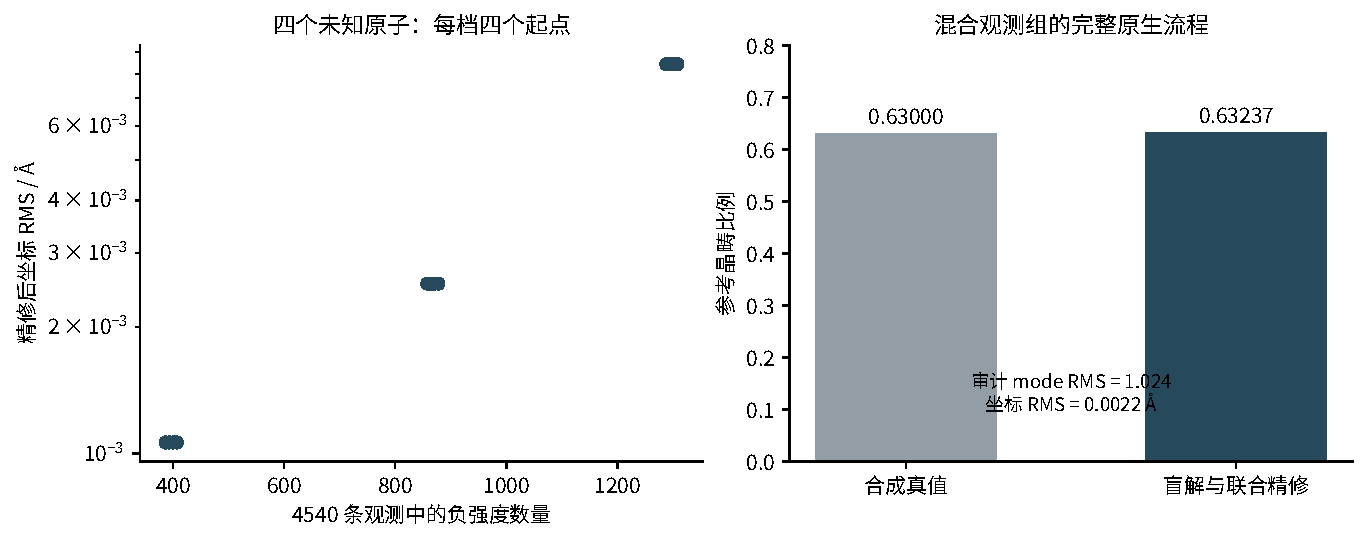
\includegraphics[width=0.92\textwidth]{figures/09_blind_recovery.pdf}
\caption{完整教材中的合成验证图。左侧为四原子盲解的不同噪声条件；右侧为含重叠观测的闭环恢复。没有提供真值坐标作为求解初值。}
\end{figure}

\section{运行入口}
安装完整源码包中的两个 Python 项目，然后运行提供的 JSON 示例：
\begin{lstlisting}
ariadne-xtal run examples/v08/solve_observations.json --root examples/v08
\end{lstlisting}
此动作也可通过 JSONL、MCP 或持久化 Ariadne 的 \code{native.run} 调用。若已有可靠结构，用 \code{structure} 输入作为初始模型，仍执行共同观测拟合和预留评价。完全缺少可用初始化证据时，流程说明缺少什么，不制造相位测量。

\section{对真实 MOF 的下一步}
预先固定组成和候选化学模型；在独立扫描块上比较预测似然，检查比例、缺陷参数的零空间及先验敏感性。几何、轮廓和吸收须在外层划分后重新标定，才能验证原始图像全流程。每个观测区域只计入目标一次；理想结构以候选或限制形式进入。
\backmatter
\begin{thebibliography}{99}
\small\linespread{1.0}\selectfont\setlength{\itemsep}{2pt}\setlength{\parskip}{0pt}
\bibitem{dials2018} Winter G, Waterman D G, Parkhurst J M, et al. DIALS: implementation and evaluation of a new integration package. Acta Crystallographica D, 2018, 74: 85--97. \href{https://doi.org/10.1107/S2059798317017235}{doi:10.1107/S2059798317017235}.
\bibitem{scaling2020} Beilsten-Edmands J, Winter G, Gildea R, et al. Scaling diffraction data in the DIALS software package: algorithms and new approaches for multi-crystal scaling. Acta Crystallographica D, 2020, 76: 385--399. \href{https://doi.org/10.1107/S2059798320003198}{doi:10.1107/S2059798320003198}.
\bibitem{sayre1952} Sayre D. The squaring method: a new method for phase determination. Acta Crystallographica, 1952, 5: 60--65. \href{https://doi.org/10.1107/S0365110X52000137}{doi:10.1107/S0365110X52000137}.
\bibitem{cochran1955} Cochran W. Relations between the phases of structure factors. Acta Crystallographica, 1955, 8: 473--478. \href{https://doi.org/10.1107/S0365110X55001485}{doi:10.1107/S0365110X55001485}.
\bibitem{karle1956} Karle J, Hauptman H. A theory of phase determination for the four types of non-centrosymmetric space groups $1P222$, $2P22$, $3P_12$, $3P_22$. Acta Crystallographica, 1956, 9: 635--651. \href{https://doi.org/10.1107/S0365110X56001741}{doi:10.1107/S0365110X56001741}.
\bibitem{snb1994} Miller R, Gallo S M, Khalak H G, Weeks C M. SnB: crystal structure determination via shake-and-bake. Journal of Applied Crystallography, 1994, 27: 613--621. \href{https://doi.org/10.1107/S0021889894000191}{doi:10.1107/S0021889894000191}.
\bibitem{charge2004} Oszlányi G, {\latintext Sütő} A. Ab initio structure solution by charge flipping. Acta Crystallographica A, 2004, 60: 134--141. \href{https://doi.org/10.1107/S0108767303027569}{doi:10.1107/S0108767303027569}.
\bibitem{charge2008} Oszlányi G, {\latintext Sütő} A. The charge flipping algorithm. Acta Crystallographica A, 2008, 64: 123--134. \href{https://doi.org/10.1107/S0108767307046028}{doi:10.1107/S0108767307046028}.
\bibitem{shelxt2015} Sheldrick G M. SHELXT -- Integrated space-group and crystal-structure determination. Acta Crystallographica A, 2015, 71: 3--8. \href{https://doi.org/10.1107/S2053273314026370}{doi:10.1107/S2053273314026370}.
\bibitem{shelxl2015} Sheldrick G M. Crystal structure refinement with SHELXL. Acta Crystallographica C, 2015, 71: 3--8. \href{https://doi.org/10.1107/S2053229614024218}{doi:10.1107/S2053229614024218}.
\bibitem{french1978} French S, Wilson K. On the treatment of negative intensity observations. Acta Crystallographica A, 1978, 34: 517--525. \href{https://doi.org/10.1107/S0567739478001114}{doi:10.1107/S0567739478001114}.
\bibitem{golub1973} Golub G H, Pereyra V. The differentiation of pseudo-inverses and nonlinear least squares problems whose variables separate. SIAM Journal on Numerical Analysis, 1973, 10: 413--432. \href{https://doi.org/10.1137/0710036}{doi:10.1137/0710036}.
\bibitem{chernoff1954} Chernoff H. On the distribution of the likelihood ratio. Annals of Mathematical Statistics, 1954, 25: 573--578. \href{https://doi.org/10.1214/aoms/1177728725}{doi:10.1214/aoms/1177728725}.
\bibitem{fen4} Bykov M, Khandarkhaeva S, Fedotenko T, et al. Synthesis of FeN$_4$ at 180 GPa and its crystal structure from a submicron-sized grain. Acta Crystallographica E, 2018, 74: 1392--1395. \href{https://doi.org/10.1107/S2056989018012161}{doi:10.1107/S2056989018012161}. 本包保留公开实验强度与原始归属说明。
\bibitem{gemmi} Gemmi project. Small-molecule crystallography, symmetry and structure-factor documentation. \url{https://gemmi.readthedocs.io/}. 本次验证使用 Gemmi 0.7.5；散射表和对称表来源，及独立前向模型的交叉检查。
\bibitem{ariadne-source} Ariadne repository. \url{https://github.com/owenxyzhang-seseTJ/Ariadne}. 本次还原侧源码基线提交 \code{60a3cfb}；原生结构侧基于随工作区保留的 Ariadne-Xtal 0.1.0。0.8.0 新增代码与验证记录随本报告发布。
\bibitem{python-buffer} Python Software Foundation. Python 3.12 C API: Buffer Protocol. \url{https://docs.python.org/3.12/c-api/buffer.html}. 原生内存视图、连续性要求与缓冲区生命周期。
\bibitem{python-threads} Python Software Foundation. Python 3.12 C API: Initialization, Finalization, and Threads. \url{https://docs.python.org/3.12/c-api/init.html}. 原生计算期间的线程状态和 GIL 管理。
\bibitem{python-process} Python Software Foundation. Python 3.12: Process-based parallelism. \url{https://docs.python.org/3.12/library/multiprocessing.html}. 全新解释器与 fork 的启动差异；本版动作隔离使用全新 subprocess 解释器。
\end{thebibliography}

\end{document}
